\chapter{Future work}
\label{ch:closing}

This chapter describes the plan of tasks to be performed in order to complete the proposed research aim. The tasks are related to the research objectives. Figure \ref{fig:future-work-objectives} illustrates the parts and the research objectives whose tasks will be conducted.

%\begin{figure}[h]
%    \centering
%    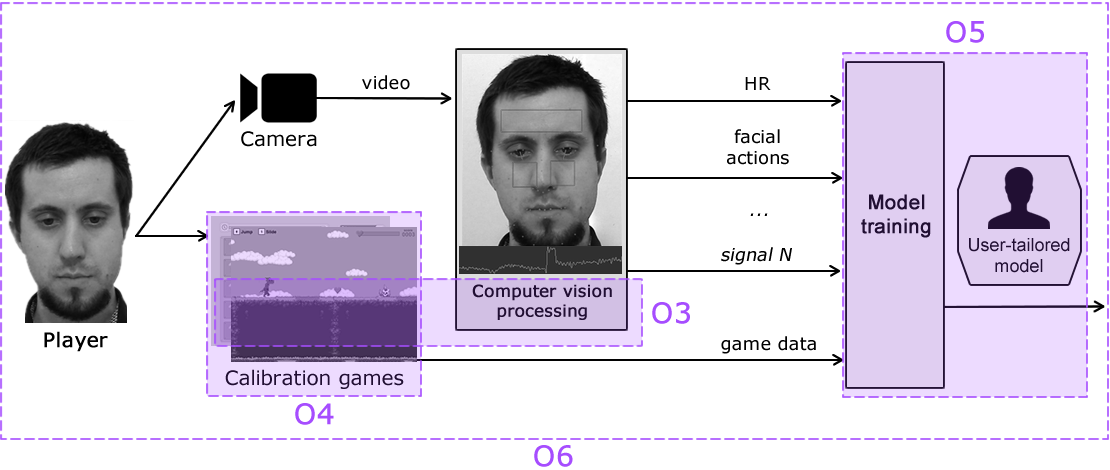
\includegraphics[width=\textwidth]{figures/future-work-objectives.png}
%    \caption{Highlight of research objectives and related parts of the solution whose tasks will be conducted as future work.}
%    \label{fig:future-work-objectives}
%\end{figure}

%The tasks involve the refinement of the process of remote acquisition of signals, definition of inputs for the user-tailored model, investigation of machine learning techniques, execution of an experiment involving emotion detection and finally the instantiation of the proposed method as a software tool. Table \ref{tab:schedule} illustrates the schedule regarding the progression of the tasks. The following sections describe the tasks in detail.
